\section{Pressure-driven electrokinetic flow}\label{sec:et:streaming_pot}
As a charged fluid is driven by a pressure gradient, a movement of
charges, i.e. an electrical current will be induced. Due to the charge
flux, a potential gradient will build up along the flow
direction. This potential is usually referred to as the streaming
potential, $\phi(\x)$, and its magnitude is determined from the
induced current through Ohm's law

\begin{equation}
\J = -  \sigma \nabla \phi  
\end{equation}   
where $\sigma$ is the conductivity of the fluid. in a perfectly
conducting fluid there will be no potential differences. Also a
complete neutral solution will carry no net current and also in this
case there will be no potential differences.

Charges under the influence of an electric field will be affected by a
force. Charges moving due to this force will, in a liquid, also pull
liquid (uncharged) molecules with them. In a macroscopic limit, the
force density affecting the charges in the liquid is assumed to affect
the liquid as a whole. The volumetric force affecting the fluid from
the presence of the streaming potential is then given by:

\begin{equation}
\F = - \rho_e \nabla \phi
\end{equation}
where $\rho_e$ is the charge density. This is an example of how the
charge density from the Nernst-Planck equation may couple to the force
term in Navier-Stokes equations. 

This force will always be affecting the fluid in a direction opposite
to the net flux of charge, i.e. the force will slow the fluid down,
this is illustrated in fig. \ref{fig:et:ev}. This effect that a moving
net charged fluid is slowed down is called the \emph{electroviscous
  effect}. The name originates from that a similar effect might be
achieved by increasing the viscosity of the fluid.

\begin{figure}
\begin{center}
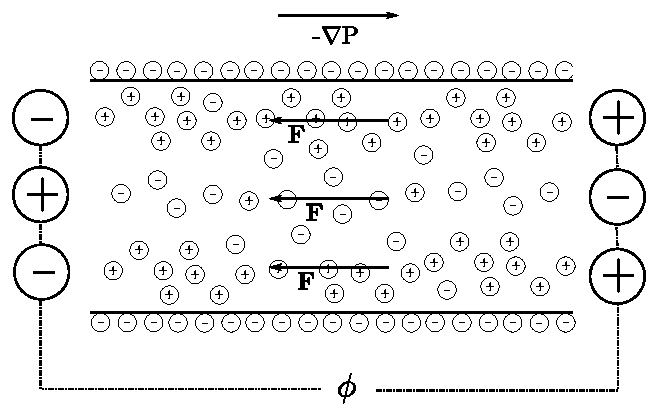
\includegraphics[width=0.7\textwidth]{fig/channel_electroviscous.pdf}
\end{center}
\caption[Example of an electroviscous system.]{Example of an
  electroviscous system. The fluid is driven by a pressure gradient,
  $\nabla \Prm$. The directions of the forces on the fluid are always
  opposite to the flow direction. The force originates from the
  potential difference, $\phi$, that builds up along the channel. The
  force is always opposite to the flow direction, thus slowing the
  flow down.}
\label{fig:et:ev}
\end{figure}
